\documentclass[../main.tex]{subfiles}

\begin{document}
    \subsubsection{Keyboard and Mouse}

    Using keyboard and mouse data posed several challenges. During the experiment, and only for the experiments, 
    we saved raw data of each of the keyboard and mouse events - for each one-second session, we saved all the events that occurred in that second. 
    In addition to the raw data, we also saved processed data. Our library processed each sequence of events within one second (a session). 
    We can see some of the features we used here \ref{table:keyboard_mouse_features} 
    and in [\ref{fig:left_click_single}, \ref{fig:left_ckick_multi}] we can see an example of the relationship between the features and the users valance. 
    In addition, we also retrieved meta-information about the use of the computer, 
    such as the number of windows switched, main window, type of window. This information was given to every keyboard/mouse model. 
    We collected this data to help the model identify the type of activity the user is performing, which might put in context the user's usage of 
    the keyboard and mouse.
 
    \begin{table}[htp]
        \centering
        \begin{tabular}{cc}
        \toprule
        Keyboard Features        & Mouse Features            \\ \midrule
        typing speed             & right click count         \\
        active typing speed      & scroll speed              \\
        average press duration   & double click count        \\
        average down to down     & cursor x distance         \\
        regular press count      & average momentary speed x \\
        punctuations press count & average speed x           \\
        space counter            & speed std                 \\
        error corrections        & std cursor angle          \\
        mode key                 & average active speed x    \\
        idle time                & idle time                 \\
        unique\_events           & right click duration      \\ \bottomrule
        \end{tabular}
        \caption{Some of the keyboard and mouse features we used.}
        \label{table:keyboard_mouse_features}
    \end{table}

    \begin{figure}[htp]
        \centering
        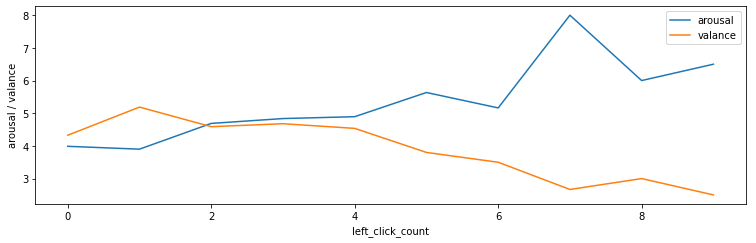
\includegraphics[width=\textwidth]{figures/left_click_single}   
        \caption{Here we can see that for one of the users clicking the left mouse button more corrolates to higher arousal, and lower valance.}
        \label{fig:left_click_single} 
    \end{figure}

    \begin{figure}[htp]
        \centering
        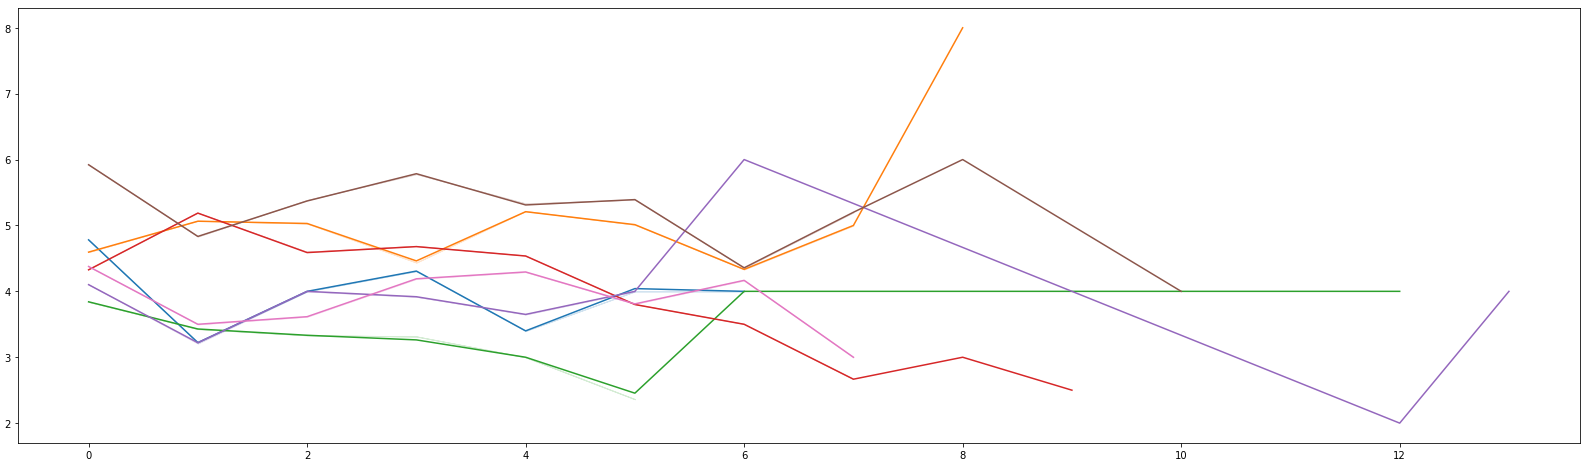
\includegraphics[width=\textwidth]{figures/left_click_multi}   
        \caption{This plot shows valance as a function of left click count, with the different colors representing different participants.
                 We can see that not all users have the same corrolation between valance and valance we have seen in \ref{fig:left_click_single} for most 
                 we can see consistent trend.}
        \label{fig:left_ckick_multi} 
    \end{figure}

    When we reached the stage of building the various models, we saw that the keyboard and mouse data was relatively dirty. 
    Therefore, after conducting the experiments, we first had to search for inconsistencies and outliers and try to find their root cause to fix them. 
    For example, some features that should be positive came out with some negative values due to inconsistencies during the data collection level.
    The raw data we collected needed to be condensed into sessions for which we could calculate our features. We chose to try three different session lengths, 
    which we used throughout the model training process - 1, 5, 10, to find the best session length for later use.
    
    We conducted feature extraction using the processors from our library for each different session duration and cleaned the results. 
    With the cleaned data and features, we could start looking at models. First, we had to separate the models into two categories, 
    classification models for the categorical and positive/negative label types and regression models used for the valance, arousal, and dominance label types.

    \begin{table}[htp]
        \centering
        \begin{tabular}{cc}
            \toprule
            classification      & regression              \\ \midrule
            Bagging             & SVR                     \\
            AdaBoost            & Lars                    \\
            Linear SVM          & Ridge                   \\
            KNN                 & Lasso                   \\
            Decision Tree       & ElasticNet              \\
            Random Forest       & Bagging Regressor       \\
            Logistic Regression & AdaBoost Regressor      \\
            Voting Classefier   & Random Forest Regressor \\
                                & Voting Regressor        \\ \bottomrule
            \end{tabular}            
            \caption{Models we trained on keyboard and mouse data.}
            \label{table:classic_models}
    \end{table}

    We trained all these models using the mouse data, using the keyboard data, 
    and using both at once. All this we did for each participant, resulting in hundreds of models. We tried to use different approaches to balance 
    the data during training, like SMOTE and ADASYN, but we saw it did not improve our results and even lower them, so we decided not to use them after all.
    On top of that, we also performed hyper-parameter tunning using optuna \cite{optuna} with hundreds of trials for each model. 
    Finally, we used six linodes with dedicated four-core CPUs to quickly train all these models, each training model for different 
    participants in parallel. The training process took approximately three days, with models of some participants finishing sooner and others later.

    \newpage

    \subsubsection{Face}

    As discussed in the literature review \ref{section:fer} we attempted to implement variants of Emotion Net Nano
    \cite{emotionnet-nano} and the Frame Attention architecture \cite{fan}. 
    We decided only to implement these two models since we had limited time and compute resources, 
    and they seemed to be the most promising. As for our implementation, we did not change much from the original papers. 
    The only changes made for both models were in the last prediction layer. We changed the number of units from 7 to 6 to 
    fit the categories we have chosen for our categorical models. For the positive/negative models, we used a Dense layer with 
    two units and a softmax activation. As for the VAD models, we decided to predict all three dimensions with a single model, 
    not to train three times the number of models. Hopefully, this way, the model could learn a better to predict the three dimensions together.

    When testing the models with a subset of the data we collected,
    we saw virtually no improvement in accuracy for the Frame Attention models over the Emotion Net models. We eventually 
    decided that we prefer only to train the Emotion Net models as they are both much faster to train and fit our goal of being very 
    small and able to run on a user's machine. Finally, we trained our Emotion Net Nano based models on each participant's data, 
    with three different session lengths (1, 5, 10), and of course trained three models for each of these combinations, 
    one to predict categorical labels, one to predict positive/negative labels, and one to predict VAD labels. 

    The image data we collected using our collection system came in sessions containing around five images each when using a session length of 1 second. 
    We processed the image data inside our collection system. We first dropped the RGB color space, leaving only black and white images, 
    then applied a filter to heighten the brightness, and finally used a face detection model from dlib \cite{dlib} which returned facial landmarks. 
    We then used said landmarks to cut out only the user's face from the image to remove noise. Because the Emotion Net model works on single images, 
    all we had to do in preprocessing was flatten the data, scale the images to (48, 48) and normalize the color data from 0-255 to 0-1.

    To evaluate our models, we used ten-fold cross-validation, which means that we trained ten different models for each of 
    the possibilities described above. In total, this comes out to be around 700 models trained. Additionally we used the predictions
    of all the models trained in the ten folds to present an ensemble classification or regression. For the ensemble method we used a 
    mean classefier or regressor depending on the models. 
    We trained each model with 100 epochs with about 4000 examples and a batch size of 100. We used different GPUs to trained these models, 
    including K80s P4s and P100s depending on availability. Unique models took around 2 minutes to train on average.

    \subsubsection{Ensemble} \label{section:methodology_ensemble}
    We made several ensemble models to assess the possibility of models combining both keyboard/mouse data and facial data. 
    We tried to see if using all three channels can increase the accuracy and improve the results. We retrieved the best three models from the 
    mouse and the keyboard channels and the Neural Network model from the camera channel. We took the probability from each model per each categorical emotion. 
    First, we tried to make a weighted average between all the models' probabilities when the Neural Network had the highest weight. 
    We knew that the Neural Network has better results than the keyboard/mouse models,
    so we wanted to check if the other models can help determine the correct label on close probabilities. 
    Then, we tried to take the maximum probability for each categorical emotion from all the models. We wanted to check whether the 
    most confident label from all models is usually the correct one.
\end{document}